\subsection{$ G$の実階数が1の場合}

\begin{thm}\label{thm:1216-main}
  $G$を実階数1の実線型半単純Lie群,$H$を$G$の非コンパクトな閉部分Lie群で,$G$のCartan対合$\Theta$に対して$\Theta H = H$かつ$\dim \ha\cap\pe = 1$とするとき,\Cref{prob:1121}が成り立つ.
\end{thm}

\begin{thm}\label{thm:0810}(\cite[p.~409, Theorem~3.1]{hel01},$\SU(2,1) $-reduction)
  $\ge = \ka \oplus \pe$を実半単純Lie環$\ge$のCartan対合$\theta$に対する Cartan分解とし,$\alpha,2\alpha\in \Sigma(\ge,\ah) $と仮定する.$0\neq X_{\alpha}\in \ge_{\alpha} $,$0\neq X_{2\alpha}\in \ge_{2\alpha} $を任意に固定したとき,$X_{\alpha},X_{2\alpha}, \theta X_{\alpha}, \theta X_{2\alpha} $から生成されるLie環$\ge^{*} $は$\sulie(2,1)$と同型である.
  
\end{thm}
以下で\Cref{thm:0810}を示すための補題や記号を設定し,\Cref{thm:0810}を示す.
\begin{nttdef}\label{nttdef:su21-red}
  \leavevmode
  \vspace{-1em}
  \begin{itemize}
  \item $\ah \subset \ge$を極大分裂可換部分代数,$\emm \defeq \zet_{\ka}(\ah) \defeq \{W\in \ka\mid [W,\ah] = \{0\} \} $とする.$B$を$\ge$のKilling 形式とする.
  \item $\Sigma(\ge,\ah) $を$\ah$に関する制限ルート系とする.$\ge_{\lambda} $を$\lambda\in \ah^{*}$のルート空間とする.
  \item $Y_{\alpha}\defeq [\theta X_{\alpha}, X_{2\alpha}] $とする.
  \item $A_{\alpha}\in \ah $を,任意の$H\in \ah$に対して$B(H,A_{\alpha}) = \alpha(H) $を満たす元とする.
    
    このとき,任意の$H\in \ah$に対して$B(H, [X_{\alpha}, \theta X_{\alpha}]) = \alpha(H) B(X_{\alpha}, \theta X_{\alpha}) $である.したがって
      \begin{align*}
        [X_{\alpha}, \theta X_{\alpha}] &= B(X_{\alpha}, \theta X_{\alpha})A_{\alpha} ,\\
        [Y_{\alpha}, \theta Y_{\alpha}] &= B(Y_{\alpha}, \theta Y_{\alpha})A_{\alpha}, \\
        [X_{2\alpha}, \theta X_{2\alpha}] &= 2B(X_{2\alpha}, \theta X_{2\alpha})A_{\alpha} 
      \end{align*}
    である.
    \item $c_{\alpha}\defeq \sqrt{\dfrac{-2}{\alpha(A_{\alpha})B(X_{\alpha}, \theta X_{\alpha})}} $,$ c_{2\alpha}  \defeq \sqrt{\dfrac{-2}{\alpha(A_{\alpha})B(X_{2\alpha}, \theta X_{2\alpha})}} $とし,
      \begin{align*}
        X_{\alpha}^{*} &\defeq c_{\alpha}X_{\alpha}, \\
        X_{2\alpha}^{*} &\defeq c_{2\alpha}X_{2\alpha},\\ 
        Y_{\alpha}^{*} &\defeq [\theta X_{\alpha}^{*}, X_{2\alpha}^{*} ] = c_{\alpha}c_{2\alpha}Y_{\alpha} ,\\
        A_{\alpha}^{*} &\defeq \dfrac{1}{12\alpha(A_{\alpha}) % \lyama \alpha, \alpha\ryama
      }A_{\alpha} 
      \end{align*}
    とする.
  \end{itemize}
\end{nttdef}

\begin{lem}\label{lem:3.2}
  $c \defeq 2\alpha(A_{\alpha})B(X_{\alpha},\theta X_{\alpha}) $とすると,$[X_{\alpha}, Y_{\alpha}] = cX_{2\alpha} $である.特に$0\neq Y_{\alpha}\neq X_{\alpha} $である.
\end{lem}
\begin{npfwn}[\Cref{lem:3.2}]
  Jacobi恒等式と$Y_{\alpha}$の定義より
  \begin{align*}
    0 &= [X_{\alpha},[\theta X_{\alpha}, X_{2\alpha}]] + [\theta X_{\alpha},[X_{2\alpha}, X_{\alpha}]] + [X_{2\alpha},[X_{\alpha}, \theta X_{\alpha}]] \\
      &= [X_{\alpha}, Y_{\alpha}] + [X_{2\alpha},B(X_{\alpha},\theta X_{\alpha})A_{\alpha}]
  \end{align*}
  であり,$3\alpha\nin \Sigma(\ge,\ah) $より第二項が0となることから\Cref{lem:3.2}が従う.
\end{npfwn}

\begin{lem}\label{lem:3.3}
  $[X_{\alpha},\theta Y_{\alpha}]\in \emm\setminus\{0\} $である.また$[[X_{\alpha}, \theta Y_{\alpha}], X_{\alpha}] = -3\alpha(A_{\alpha})B(X_{\alpha}, \theta X_{\alpha})Y_{\alpha} $である.
\end{lem}

\begin{npfwn}[\Cref{lem:3.3}]
  $Y_{\alpha} \in \ge_{\alpha} $より$[X_{\alpha},\theta Y_{\alpha}]\in \emm+ \ah$であり,任意の$H\in \ah$に対して
  \begin{align*}
    B(H, [X_{\alpha},\theta Y_{\alpha}]) &= B([H, X_{\alpha}], Y_{\alpha}) = \alpha(H) B(X_{\alpha}, [X_{\alpha}, \theta X_{2\alpha}]) \\
                                         &= \alpha(H)B([X_{\alpha}, X_{\alpha}], X_{2\alpha}) \\
                                         &= 0
  \end{align*}
  であることより$[X_{\alpha},\theta Y_{\alpha}]\in \emm$である.

  さらに,
  \begin{align*}
    [[\theta X_{\alpha},Y_{\alpha}], X_{\alpha}] &= -[[Y_{\alpha}, X_{\alpha}], \theta X_{\alpha}] - [[X_{\alpha}, \theta X_{\alpha}], Y_{\alpha}]\\
                                                 &= c[X_{2\alpha}, \theta X_{\alpha}] -  B(X_{\alpha},\theta X_{\alpha})\alpha(A_{\alpha})Y_{\alpha}\\
                                                 &= -cY_{\alpha}-  B(X_{\alpha},\theta X_{\alpha})\alpha(A_{\alpha})Y_{\alpha} \\
                                                 &= -3\alpha(A_{\alpha})B(X_{\alpha}, \theta X_{\alpha})Y_{\alpha} \neq 0
  \end{align*}
  より,$\theta [\theta X_{\alpha},Y_{\alpha}] = [X_{\alpha},\theta Y_{\alpha}]\in \emm\setminus\{0\} $である.
\end{npfwn}

\vspace{-1em}
\begin{lem}\label{lem:3.4}  
  $\real X_{\alpha} + \real Y_{\alpha} $は$\ad_{\ge}([X_{\alpha}, \theta Y_{\alpha}]) $で不変である.  
  さらに
  \begin{align*}
    [[X_{\alpha}, \theta Y_{\alpha}], Y_{\alpha}] &= -6\alpha(A_{\alpha})^2B(X_{\alpha}, \theta X_{\alpha})B(X_{2\alpha}, \theta X_{2\alpha})X_{\alpha},\\
  [Y_{\alpha}, \theta Y_{\alpha}] &= -2\alpha(A_{\alpha})B(X_{\alpha}, \theta X_{\alpha})B(X_{2\alpha}, \theta X_{2\alpha})A_{\alpha}
  \end{align*}
  である.

\end{lem}

\begin{npfwn}[\Cref{lem:3.4}]
  $[[X_{\alpha}, \theta Y_{\alpha}], Y_{\alpha}]  \in \real X_{\alpha} $を示せば,\Cref{lem:3.3}と併せて\Cref{lem:3.4}が従う.

  
  \begin{align*}
    [[X_{\alpha}, \theta Y_{\alpha}], Y_{\alpha}] &= -[[\theta Y_{\alpha}, Y_{\alpha}], X_{\alpha}] - [[Y_{\alpha}, X_{\alpha}], \theta Y_{\alpha}] \\
                                                  &= B(Y_{\alpha}, \theta Y_{\alpha})\alpha(A_{\alpha})X_{\alpha} +c[X_{2\alpha},[X_{\alpha}, \theta X_{2\alpha}]] \\
                                                  &= B(Y_{\alpha}, \theta Y_{\alpha})\alpha(A_{\alpha})X_{\alpha} - c[X_{\alpha}, [\theta X_{2\alpha}, X_{2\alpha}]] - c[\theta X_{2\alpha},[X_{2\alpha},X_{\alpha}]] \\
                                                  &= B(Y_{\alpha}, \theta Y_{\alpha})\alpha(A_{\alpha})X_{\alpha} - cB(X_{2\alpha},\theta X_{2\alpha})\alpha(A_{2\alpha})X_{\alpha}
  \end{align*}
  であり ($ \ge_{3\alpha} = \{0\} $による),$A_{2\alpha} = 2A_{\alpha} $であるから,
  \begin{align*}
[[X_{\alpha}, \theta Y_{\alpha}], Y_{\alpha}] =  B(Y_{\alpha}, \theta Y_{\alpha})\alpha(A_{\alpha})X_{\alpha} - 4\alpha(A_{\alpha})^2B(X_{\alpha}, \theta X_{\alpha})B(X_{2\alpha}, \theta X_{2\alpha})X_{\alpha}
  \end{align*}
  を得る.

  さらに,
  \begin{align*}
    B(Y_{\alpha}, \theta Y_{\alpha}) &= B(Y_{\alpha},[X_{\alpha}, \theta X_{2\alpha}]) = -B([X_{\alpha}, Y_{\alpha}], \theta X_{2\alpha}) \\
                                     &= -2\alpha(A_{\alpha})B(X_{\alpha},\theta X_{\alpha})B(X_{2\alpha}, \theta X_{2\alpha})
  \end{align*}
  であるから,最終的に
  \begin{align*}
    [[X_{\alpha}, \theta Y_{\alpha}], Y_{\alpha}] &=  B(Y_{\alpha}, \theta Y_{\alpha})\alpha(A_{\alpha})X_{\alpha} - 4\alpha(A_{\alpha})^2B(X_{\alpha}, \theta X_{\alpha})B(X_{2\alpha}, \theta X_{2\alpha})X_{\alpha} \\
                                                  &= -6\alpha(A_{\alpha})^2B(X_{\alpha}, \theta X_{\alpha})B(X_{2\alpha}, \theta X_{2\alpha})X_{\alpha}
  \end{align*}
を得る.  
\end{npfwn}

\begin{lem}\label{lem:3.5}
  $[[X_{\alpha}, \theta Y_{\alpha}], X_{2\alpha}] = 0$である.
\end{lem}
\begin{npfwn}[\Cref{lem:3.5}]
  \Cref{lem:3.2}--\ref{lem:3.4}とJacobi恒等式による.具体的には,$T\defeq [X_{\alpha},\theta Y_{\alpha}] $とすると,\Cref{lem:3.3}と\Cref{lem:3.4}よりそれぞれ
  \begin{align}
    [T, X_{\alpha}] \in \real Y_{\alpha} ,\ [T, Y_{\alpha}] \in \real X_{\alpha}\label{eq:lem3.5}
  \end{align}
  である.Jacobi恒等式より
  \begin{align}
    [T, [X_{\alpha},Y_{\alpha}]] = -[X_{\alpha},[Y_{\alpha},T]] - [Y_{\alpha},[X_{\alpha},T]]\label{eq:lem3.5-2}
  \end{align}
  であり,\Cref{eq:lem3.5}より\Cref{eq:lem3.5-2}の右辺は0となる.\Cref{lem:3.2}より$[X_{\alpha}, Y_{\alpha}] = cX_{2\alpha} $であり,これを用いることで\Cref{lem:3.5}の主張を得る.
\end{npfwn}

\begin{lem}\label{lem:3.6}
  $[Y_{\alpha},\theta X_{2\alpha}] = 2\alpha(A_{\alpha})B(X_{2\alpha}, \theta X_{2\alpha})\theta X_{\alpha} $である.  
\end{lem}
\begin{npfwn}[\Cref{lem:3.6}]
  Jacobi恒等式を用いて与式を変形し計算することにより示せる.
\end{npfwn}



\begin{npfwn}[\Cref{thm:0810}]
  $\ge^{*}_0 \defeq \real A_{\alpha}\oplus \real[X_{\alpha}, \theta Y_{\alpha}] $,$\ge^{*}_{\alpha} \defeq \real X_{\alpha}\oplus \real Y_{\alpha}  $,$\ge^{*}_{-\alpha} \defeq \real \theta X_{\alpha}\oplus \real \theta Y_{\alpha}  $,$\ge^{*}_{2\alpha} \defeq \real X_{2\alpha} $,$\ge^{*}_{-2\alpha} \defeq \real \theta X_{2\alpha}$とすると,\Cref{lem:3.2}--\ref{lem:3.6}より,$\ge^{*} = \ge^{*}_{0} \oplus \ge^{*}_{\alpha}\oplus \ge^{*}_{-\alpha} \oplus \ge^{*}_{2\alpha} \oplus \ge^{*}_{-2\alpha} $が示される.

  
  非自明な$\ge^{*} $のLie括弧の関係は以下の通りである (残りの関係式はこの両辺に$\theta$をつけることで得られる).

  
  \begin{align*}
    [X_{\alpha}^{*}, Y_{\alpha}^{*}] &= -4X_{2\alpha}^{*}, &\text{(\Cref{lem:3.2}による)},\\
    [X_{\alpha}^{*},[X_{\alpha}^{*}, \theta Y_{\alpha}^{*}]]  &= -6Y_{\alpha}^{*}, &\text{(\Cref{lem:3.3}による)},\\
    [X_{\alpha}^{*}, \theta X_{\alpha}^{*}] &= -24A_{\alpha}^{*}, & (定義による),\\
    [X_{\alpha}^{*},X_{2\alpha}^{*}] &= 0, &\text{($\ge_{3\alpha} = 0$による)},\\
    [X_{\alpha}^{*}, \theta X_{2\alpha}^{*}] &= \theta Y_{\alpha}^{*} ,& (定義による)\\
    [Y_{\alpha}^{*},X_{2\alpha}^{*}] &= 0, &\text{(\Cref{lem:3.5}による)},\\
    [Y_{\alpha}^{*},\theta X_{2\alpha}^{*}] &= -4\theta X_{\alpha}^{*} , &\text{(\Cref{lem:3.6}による)},\\
    [Y_{\alpha}^{*}, \theta Y_{\alpha}^{*}] &= -96A_{\alpha}^{*} , &\text{(\Cref{lem:3.4}による)},\\
    [Y_{\alpha}^{*}, [X_{\alpha}^{*}, \theta Y_{\alpha}^{*}]] &= 24X_{\alpha}^{*},  &\text{(\Cref{lem:3.4}による)},\\
    [[X_{\alpha}^{*}, \theta Y_{\alpha}], X_{2\alpha}^{*}] &= [[X_{\alpha}^{*}, \theta Y_{\alpha}], \theta X_{2\alpha}^{*}] = 0, &\text{(\Cref{lem:3.6}による)},\\
    [X_{2\alpha}^{*} ,\theta X_{2\alpha}^{*} ] &= -48A_{\alpha}^{*}, & (定義による)
  \end{align*}

  これらを踏まえて$\ge^{*} $と$\sulie(2,1) $の対応を,
  \begin{align*}
    X_{\alpha}^{*} & \leftrightarrow
                     \begin{pmatrix}
                       0 & 1 & 0\\ -1 & 0 & 1\\ 0 & 1 & 0
                     \end{pmatrix},&   X_{2\alpha}^{*}  \leftrightarrow
                     \begin{pmatrix}
                       \img & 0 & -\img \\ 0 & 0 & 0\\ \img & 0 & -\img
                     \end{pmatrix},\\
    \theta X_{\alpha}^{*} & \leftrightarrow
                     \begin{pmatrix}
                       0 & 1 & 0\\ -1 & 0 & -1\\ 0 & -1 & 0
                     \end{pmatrix},&   \theta X_{2\alpha}^{*}  \leftrightarrow
                     \begin{pmatrix}
                       \img & 0 & \img \\ 0 & 0 & 0\\ -\img & 0 & -\img
                     \end{pmatrix},\\
    Y_{\alpha}^{*} & \leftrightarrow
                     -2 \begin{pmatrix}
                       0 & \img & 0\\ \img & 0 & -\img \\ 0 & \img & 0
                     \end{pmatrix},&   \theta Y_{\alpha}^{*}  \leftrightarrow
                     \begin{pmatrix}
                       0 & \img  & 0 \\ \img & 0 & \img \\ 0 & -\img & -0
                     \end{pmatrix},\\
    A_{\alpha}^{*} & \leftrightarrow
                    \frac{1}{12} \begin{pmatrix}
                       0 & 0 & 1\\ 0 & 0 & 0\\ 1 & 0 & 0
                     \end{pmatrix},&   [X_{\alpha},\theta Y_{\alpha}^{*}] \leftrightarrow
                    -4 \begin{pmatrix}
                       \img & 0 & 0 \\ 0 & -2\img & 0\\  & 0 & \img
                     \end{pmatrix}
  \end{align*}
  でつける.この対応がLie環としての同型であること (上の関係式が満たされること) は計算することにより従う.

  以上より\Cref{thm:0810}が示された.  
\end{npfwn}

\begin{lem}\label{lem:su11}
  
  $\Sigma(\ge,\ah) = \{\pm\alpha\}$の場合,任意に固定した$0\neq X_{\alpha}\in \ge_{\alpha}$と$\theta X_{\alpha}$により生成される部分Lie環$\ge'$は$\sulie(1,1)$と同型である.
\end{lem}

\begin{npfwn}[\Cref{lem:su11}]
  $\ge_{2\alpha} = \ge_{-2\alpha} = \{0\}  $より,$[X_{\alpha}, X_{\alpha}] = [X_{-\alpha}, X_{-\alpha}] = 0 $である. $A_{\alpha}\in \ah $を任意の$H\in \ah$に対して$B(H,A_{\alpha}) = \alpha(H) $を満たす元とする.任意の$H\in \ah$に対して$B(H, [X_{\alpha}, \theta X_{\alpha}]) = \alpha(H) B(X_{\alpha}, \theta X_{\alpha}) $である.任意の$0\neq W\in \ge$に対し$-B(W,\theta W) > 0 $より$[X_{\alpha}, \theta X_{\alpha}] = B(X_{\alpha}, \theta X_{\alpha})A_{\alpha}\neq 0 $である.

  以上より$X_{\alpha} $と$\theta X_{\alpha} $により生成される$\ge$の部分Lie環$\ge'$は$\ge' = \real A_{\alpha}\oplus \real X_{\alpha} \oplus \real X_{-\alpha}  $である.

  % $\tr(\ad_{\ge'}A_{\alpha} \ad_{\ge'}A_{\alpha} ) = 2\alpha(A_{\alpha})^2\neq 0 $より,
  $c_{\alpha}\defeq \dfrac{2}{\alpha(A_{\alpha})} $を用いて$\ge'$と$\sulie(1,1)$の対応を
  \begin{align*}
    % \dfrac{1}{\alpha(A_{\alpha})}
    A_{\alpha} &\leftrightarrow
    \begin{pmatrix}
      0 & 1 \\ 1 & 0
    \end{pmatrix},&  c_{\alpha} X_{\alpha} \leftrightarrow
      \begin{pmatrix}
        \sqrt{-1} & -\sqrt{-1} \\ \sqrt{-1} & -\sqrt{-1}
      \end{pmatrix},\\
    c_{\alpha}X_{-\alpha} &\leftrightarrow
      \begin{pmatrix}
        \sqrt{-1} & \sqrt{-1} \\ -\sqrt{-1} & -\sqrt{-1}
      \end{pmatrix} 
  \end{align*}
  により与えると,これは$\ge'$と$\sulie(1,1)$の間の同型になっている.
\end{npfwn}

\begin{cor}\label{cor:sub-lie-alg}
  $G$を実階数1の実半単純Lie群とする.任意の$0\neq Y\in \pe\cap\ha$と任意の$X\in \pe\setminus \ha$を固定したとき,$X,Y$を含む部分Lie環$\ge_0\subset \ge$で,$\ge_0\simeq \sulie(1,1) $か$\ge_0\simeq \sulie(2,1)$なるものが存在する.
\end{cor}

\begin{npfwn}[\Cref{cor:sub-lie-alg}]
  $G$は実階数1より,極大分裂可換部分代数$\ah\defeq \real Y\subset \ge$に対しある$\alpha\in \ah^{*} $が存在して$\Sigma(\ge,\ah) = \{\pm\alpha\} $あるいは$\Sigma(\ge,\ah)  = \{\pm\alpha, \pm 2\alpha \} $であるから,それぞれ\Cref{thm:0810}と\Cref{lem:su11}より\Cref{cor:sub-lie-alg}の主張が従う.以下で$\Sigma(\ge,\ah)$の形で場合分けしてこの議論をを確認する.
  \begin{case}
    \textbf{$\Sigma(\ge,\ah) = \{\pm\alpha\} $の場合}

    $\ge = \ge_{0} \oplus \ge_{\alpha}\oplus \ge_{-\alpha} $,$\ge_0 \defeq \ze_{\ge}(\ah) $より$X\in  \pe\setminus \ah$をこの分解に対応して$X = X_0 + X_{\alpha} + X_{-\alpha} $と分解すると,$X\in \pe\setminus \ah$より$ X_{-\alpha} = -\theta X_{\alpha}\neq 0 $である.$Y\in \real [X_{\alpha}, \theta X_{\alpha}] $であるからこの$X_{\alpha}\neq 0 $に\Cref{lem:su11}を適用することにより$\ge_0\simeq \sulie(1,1)$で$X,Y\in \ge_0 $なるものが存在する.
    
  \end{case}
  
  \begin{case}
    \textbf{$\Sigma(\ge,\ah) = \{\pm\alpha, \pm 2\alpha\} $の場合}

    $\ge = \ge_{0} \oplus \ge_{\alpha}\oplus \ge_{-\alpha} \oplus \ge_{2\alpha}\oplus \ge_{-2\alpha}  $,$\ge_0 \defeq \ze_{\ge}(\ah) $より$X\in \pe\setminus \ah$をこの分解に対応して$X = X_0 + X_{\alpha} + X_{-\alpha} + X_{2\alpha} + X_{-2\alpha} $と書くと,$X\in \pe$より$ X_{-\alpha} = - \theta X_{\alpha} $,$ X_{-2\alpha} = - \theta X_{2\alpha} $である.

    ここで$X\nin \ah$より,
    \begin{enumerate}
    \item $X_{\alpha}\neq 0 $かつ$X_{2\alpha}\neq 0 $
    \item $X_{\alpha}\neq 0 $かつ$X_{2\alpha} =  0 $
    \item $X_{\alpha} =  0 $かつ$X_{2\alpha} \neq  0 $
    \end{enumerate}
    のいずれかである.
    \begin{enumerate}
    \item[1] の場合はこの$X_{\alpha}, X_{2\alpha} $と$Y$に,
    \item[2] の場合はこの$X_{\alpha}$と,適当な$0\neq X_{2\alpha}'\in \ge_{2\alpha} $と$Y$に,
    \item[3] の場合はこの$X_{2\alpha}$と,適当な$0\neq X_{\alpha}'\in \ge_{\alpha} $と$Y$に,
    \end{enumerate}
    \Cref{thm:0810}を適用することにより$\ge_0\simeq \sulie(2,1)$で$X,Y\in \ge_0 $なるものが存在する.    
  \end{case}   
\end{npfwn}

\Cref{cor:sub-lie-alg}で定めた$\ge_0$とその$G$における解析部分群$G_0$について次の3つが成り立つ.
\begin{lem}(\cite[p.~409, Lemma~2.2]{hel01})
  $\ge$のCartan対合$\theta$に対して$\ge_0 = \theta\ge_0$であり,$\ge_0 $への$\theta$の制限は$\ge_0$のCartan分解を与える.
\end{lem}

\begin{lem}(\cite[p.~82]{yos38})
  $G$を線型Lie群,$\ha\subset \ge$は実半単純な部分Lie環とする.このとき$\ha$の$G$における解析的部分群は閉部分群である.
\end{lem}
\begin{cor}
  \Cref{cor:sub-lie-alg}の$\ge_0$の$G$における解析的部分群を$G_0$とする.$G_0 $は$G$の閉部分群である.
\end{cor}


\begin{lem}(\cite[p.~409, Lemma~2.3]{hel01}) \Cref{cor:sub-lie-alg}の$\ge_0$の$G$における解析的部分群を$G_0$とする.$G = KAN$を$G$の岩澤分解,$G_0 = K_0A_0N_0$を$G$の岩澤分解とするとき,
  \begin{align*}
    K_0\defeq G_0\cap K,\ A_0 \defeq G_0\cap A,\ N_0\defeq G_0\cap N, 
  \end{align*}
  であり,$G_0/K_0 \simeq G_0/K$は$G/K$の全測地的な部分Riemann多様体である.
  
\end{lem}

以上のことを用いて,$G$が実階数1,$\dim \ha\cap\pe = 1 $の場合を$\SU(1,2) $ないし$\SU(1,1) $に帰着させることにより\Cref{thm:1216-main}を示す.

\begin{npfwn}[\Cref{thm:1216-main}]\bluetext{おそらく$\dim H = 1$でない場合も背理法で示せる気がする.}
  $\ge$の極大分裂可換部分代数$\ha\cap\pe$の定めるルート系を$\Sigma(\ge,\ha) $とし,$\Sigma(\ge,\ha) $の形によって2通りに場合分けして証明する.
  
  \textbf{$\Sigma(\ge,\ha) = \{\pm\alpha \}$のとき}
  
  \Cref{cor:sub-lie-alg}により$X$と$\ha\cap\pe $を含む部分Lie環$\ge' \subset \ge $で$\sulie(1,1) $に同型なものが存在する.$\ge' $に対応する$G$の解析的部分群を$G'$とし,その岩澤分解を$G' = K'A'N' $とする.このとき$e^{Z(t X)}\cdot o_K = e^{-Y(tX)}e^{tX}\cdot o_K\in G'/K $であるから$Z(tX)\in \ge'\cap \per{\ha}\cap \pe\subset \ge'\cap\pe $であり,$Y(\real X) $の有界性は全測地的的な部分Riemann多様体$G'/K'\subset G/K$に対して行えば良いことがわかる.したがって\Cref{prop:prob-eg}により$X\in\pe_{H,\bdd}$であることと$ X = 0 $あるいは$X\in \pe\setminus\ha $が同値であることが言え,\Cref{thm:1216-main}が示された.
  
  % 任意の固定した$\tau \in \real$に対し$\ah_{\tau} \defeq \real Y(\tau X)$が定める制限ルート系も,ある$\alpha_{\tau} \in \ah_{\tau}^{*}$,$ \norm{\alpha_{\tau}} = 1 $により$\Sigma(\ge,\ah_{\tau}) = \{\pm\alpha_{\tau} \}$となる.任意の$\tau,\tau'\in \real$に対し,ある$k\in K$が存在して$k\cdot \alpha_{\tau}  = \alpha_{\tau'} $であるから,$\norm{\alpha} \defeq \norm{\alpha_{\tau}} $は$\tau\in \real$に依らない.

  
  
  % \bluetext{定数を確認せよ $A_{\alpha}\in \ha $を任意の$H\in \ha $に対して$B(H,A_{\alpha}) = \alpha(H) $を満たす元とすると, 任意の固定した$\tau \in \real$に対し,$Y(\tau X) $に対応する$\ge_{\tau} $の元は$\inlineequation[eq:corresp]{\dfrac{B(Y(\tau X), A_{\alpha}) }{\norm{A_{\alpha}}}
  % \begin{pmatrix}
  %   0 & 1 \\
  %   1 & 0 
  % \end{pmatrix}}
  % $である.}
  
  % $Y(\real X) $の非有界性より,適当に列$\{t_{n}\in \real\}_{n\in \nat} $,$t_n\underset{n\to \infty}{\longrightarrow} \infty$を取ると$0 <  \norm{Y(t_n X)} = s_n $,$\forall n\in \nat$かつ$s_n\to \infty$,$n\to \infty$とできる.% さらに$Z(t_n X) = r_n Z_n $,$Z_n\in \per{\ha}\cap \pe $,$\norm{Z_n} = 1 $,$r_n\in \real$と書くと,\Cref{thm:kob97}より$\abs{r_n}\to \infty$,$n\to \infty$である.$\norm{Z_n} = 1 $より,必要なら$\{t_{n}\in \real\}_{n\in \nat} $の部分列を取ることで$\lim_{n\to \infty}Z_n = Z_{\infty}\in \per{\ha}\cap \pe $,$\norm{Z_{\infty} } = 1$なる$Z_{\infty}$が存在する.

  % 必要ならpositive systemを取り替えることで$B(Y(t_n X), A_{\alpha}) > 0$と仮定する.このとき$B(Y(t_n X), A_{\alpha}) = s_n$であるから,\Cref{eq:corresp}より$\ge'\simeq \sulie(1,1) $の同型において$Y(t_n X)  $は$s_n\begin{pmatrix}
  %   0 & 1 \\
  %   1 & 0 
  % \end{pmatrix}$に対応する.

  % 以上の性質を満たす$\{t_n\}_{n\in \nat} $,$\{s_n\}_{n\in \nat}  $% ,$\{r_n \}_{n\in \nat} $,$\{Z_{n} \}_{n\in \nat} $,$Z_{\infty} $
  % に対して

  
  \textbf{$\Sigma(\ge,\ah) = \{\pm\alpha,\pm 2\alpha \}$のとき}

  \Cref{cor:sub-lie-alg}により$X$と$\ha \cap\pe$を含む部分Lie環$\ge^* \subset \ge $で$\sulie(2,1) $に同型なものが存在する.$\ge^* $に対応する$G$の解析的部分群を$G^* $とし,その岩澤分解を$G^* = K^*A^*N^* $とする.このとき$e^{Z(t X)}\cdot o_K = e^{-Y(tX)}e^{tX}\cdot o_K\in G'/K $であるから$Z(tX)\in \ge^* \cap \per{\ha}\cap \pe\subset \ge^*\cap\pe $であり,$Y(\real X) $の有界性は全測地的的な部分Riemann多様体$G^*/K^* \subset G/K$に対して行えば良いことがわかる.したがって\Cref{prop:classical-rank-one}により$X\in\pe_{H,\bdd}$であることと$ X = 0 $あるいは$X\in \pe\setminus\ha $が同値であることが言え,\Cref{thm:1216-main}が示された.
\end{npfwn}

    % 場合1と同様に,任意の固定した$\tau \in \real$に対し$\ah_{\tau} \defeq \real Y(\tau X)$が定める制限ルート系も,ある$\alpha_{\tau} \in \ah_{\tau}^{*}$,$ \norm{\alpha_{\tau}} = 1 $により$\Sigma(\ge,\ah_{\tau}) = \{\pm\alpha_{\tau}, \pm 2\alpha_{\tau} \}$となるが,$Y(\real X) $の非有界性より,ある$T\in \real$で$\abs{\alpha_{t}(Y(tX))} >  $\bluetext{埋めよ},$\forall t \geq T$なるものが存在する.
    
    



\subsubsection{補足: \Cref{thm:1216-main}の微分幾何的側面}
\begin{defi}({\cite[Definition~1.3]{e72-1}})\label{def:visibility}
  $M$が完備かつ非正の断面曲率をもつ1-連結Riemann多様体であるとき,$M$をHadamard多様体といい,Hadamard多様体$M$が visibility manifold であるとは,$\forall p\in M, \forall \epsilon > 0$に対し,ある$r(p,\epsilon) >0 $が存在して,測地線$\gamma\colon [t_0, t_1]\to X $が任意の$ t\in [t_0, t_1]$に対し$d_{M}(p, \gamma(t))\geq r(p,\epsilon) $を満たすならば,$\measuredangle_{p}(\gamma(t_0), \gamma(t_1)) \leq \epsilon $であることである.
\end{defi}

後に示すように{\Poincare}円板はvisibility manifoldであるが,\Cref{lem:0106}よりその片鱗を見ることはできる.具体的には$ 0 <  \epsilon  < \frac{\pi}{2} $に対し$t_{\epsilon} \defeq \dfrac{1}{2}\inv{\sinh}\dfrac{1}{\abs{\tan \epsilon}} $とし,測地線$\gamma_{\epsilon}(s) = e^{t_{\epsilon} Y}e^{sZ}\cdot o_K $とすると,\Cref{lem:0106}より任意の$s_0,s_1\in \real$に対し$\measuredangle_{o_K}(\gamma_{\epsilon} (s_0), \gamma_{\epsilon} (s_1)) \leq \epsilon $である.この様子を図示すると\Cref{fig:visibility}のようになる.

\begin{figure}[H]
  \centering
  % \raggedleft
  % \raggedrightp
  % 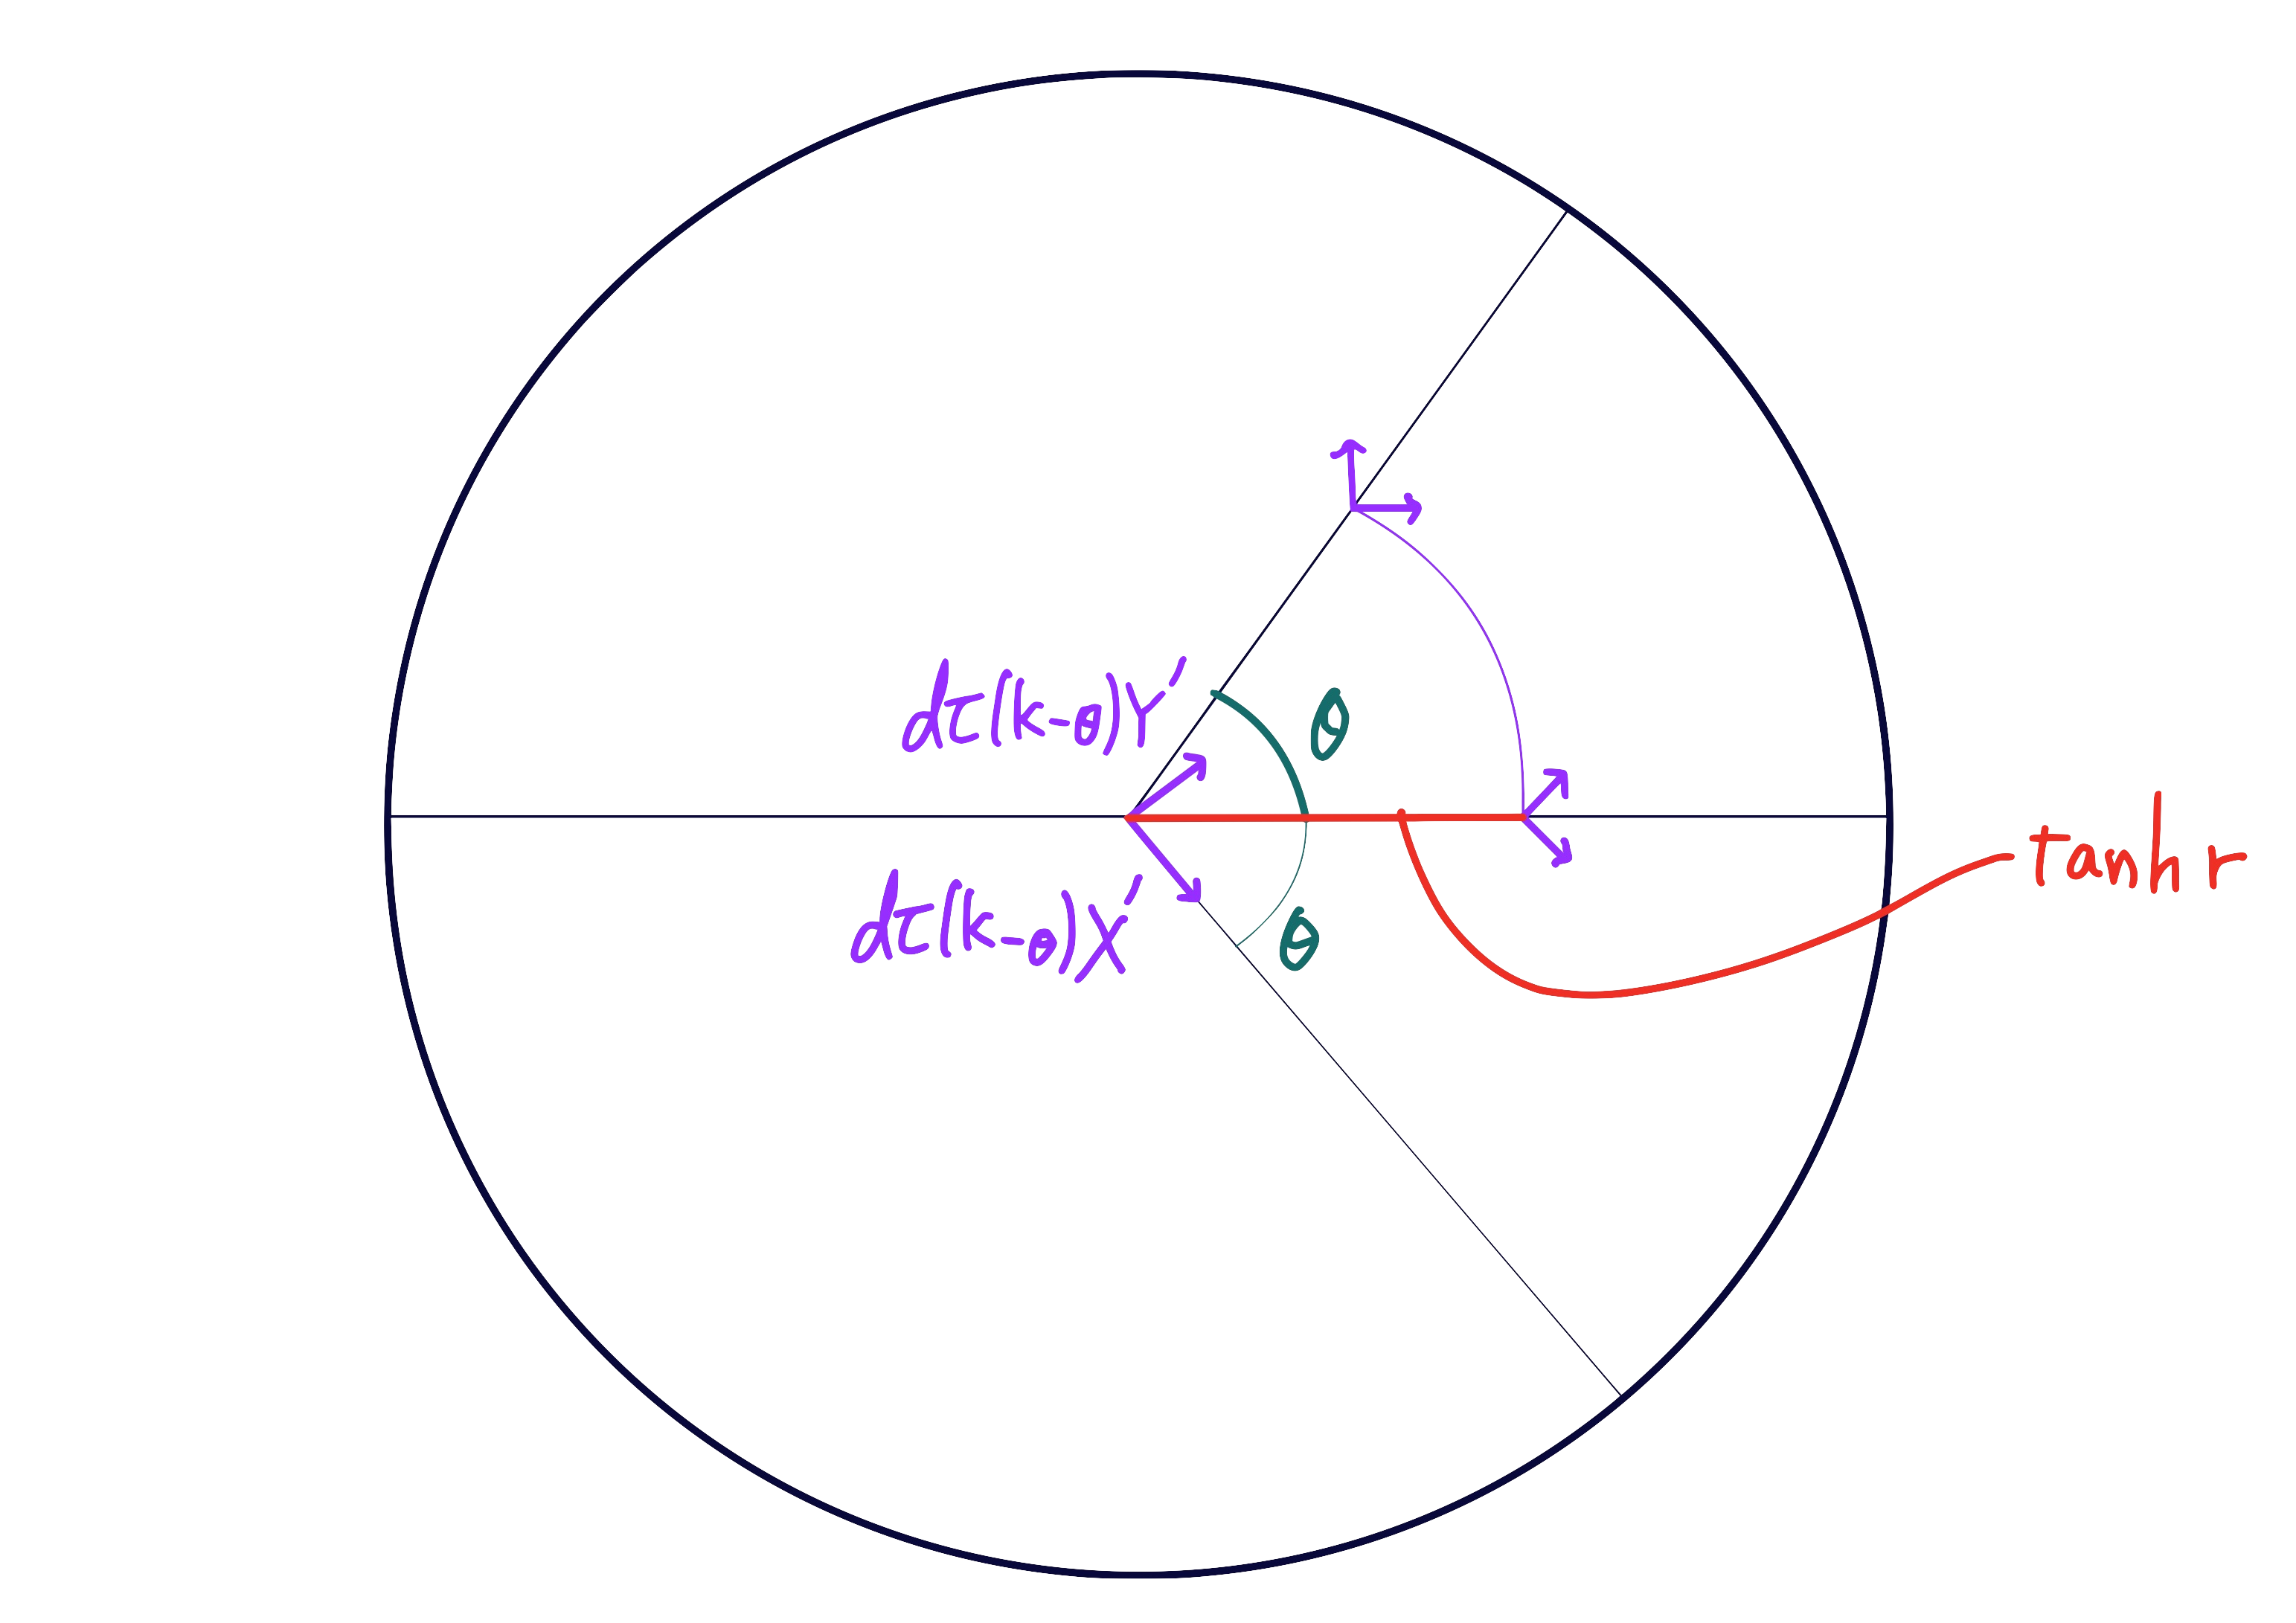
\includegraphics[scale=0.08]{../graph/riem-su11.png}
  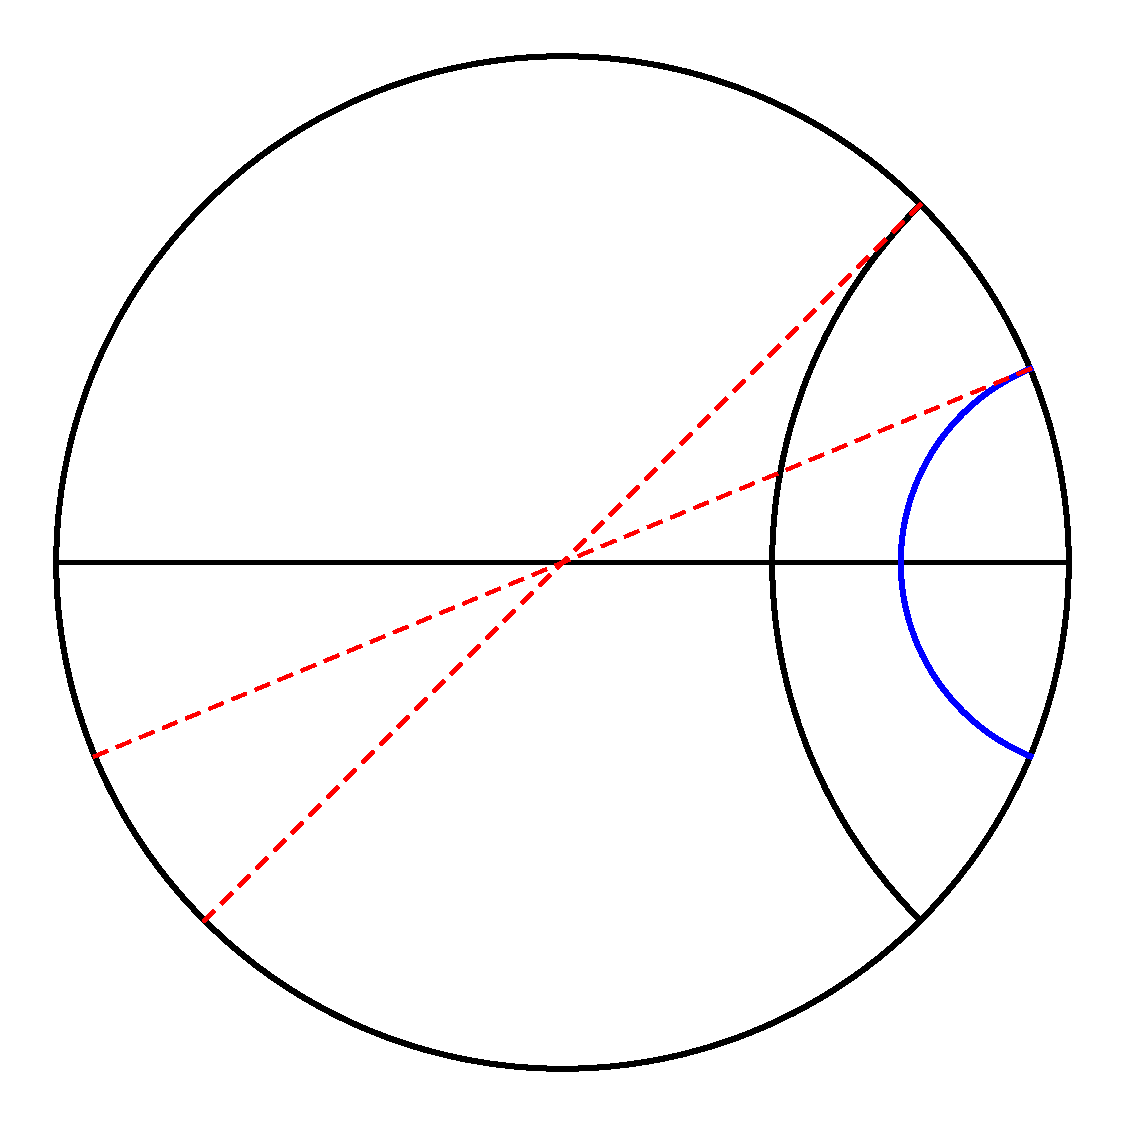
\includegraphics[scale=0.3]{../graph/visibility-2.pdf}
  \caption{visibility manifoldのイメージ}
  \label{fig:visibility}
\end{figure}


\begin{thm}({\cite[p.~296, 9.33~Theorem]{bh99}, originally \cite[Theorem~4.1]{e72-2}})\label{thm:visibility-and-rank}  
  $\exists C\cptsub M\st M = \bigcup\{f(C)\mid f\in \isom(M) \}  $なるHadamard多様体$M$に対し,次は同値である.
  \vspace{-1em}
  \begin{enumerate}
    \renewcommand{\labelenumi}{(\roman{enumi})}
  \item $M$はvisibility manifoldである.
  \item 全測地的な部分Riemann多様体$M'\subset M$で$\real^2$と等長同型なものが存在しない.
  \end{enumerate}
\end{thm}

ここでRiemann対称空間はHadamard多様体であり,\Cref{thm:visibility-and-rank}の (ii) は$G$の実階数が1以下であることと同値である.したがって$G$の実階数が1の場合$G/K$はvisibility manifoldであり,$G = \SU(1,2) $,$H= \SO(1,1)$の場合の証明と全く同様にして背理法により\Cref{prob:1121}が示される.
